\documentclass{article}

% Set page size and margins
% Replace `letterpaper' with `a4paper' for UK/EU standard size
\usepackage[letterpaper,top=2cm,bottom=2cm,left=3cm,right=3cm,marginparwidth=1.75cm]{geometry}
\usepackage[spanish]{babel}
\usepackage{url}
\usepackage{hyperref}
\usepackage{csquotes}
\usepackage{amsmath}
\usepackage{amssymb}
\usepackage{graphicx}
\usepackage{listings}
\usepackage{xcolor}
\usepackage{setspace}
\usepackage{float}

\graphicspath{ {assets/} }

%Code colors:
\definecolor{codegreen}{rgb}{0,0.6,0}
\definecolor{codegray}{rgb}{0.5,0.5,0.5}
\definecolor{codepurple}{rgb}{0.58,0,0.82}
\definecolor{backcolour}{rgb}{0.95,0.95,0.92}
\doublespacing

\lstdefinestyle{mystyle}{
    backgroundcolor=\color{backcolour},
    commentstyle=\color{codegreen},
    keywordstyle=\color{magenta},
    numberstyle=\tiny\color{codegray},
    stringstyle=\color{codepurple},
    basicstyle=\ttfamily\footnotesize,
    breakatwhitespace=false,
    breaklines=false,
    captionpos=b,
    keepspaces=true,
    numbers=left,
    numbersep=5pt,
    showstringspaces=false,
    showlines=false,
    showtabs=false,
    tabsize=2
}

\lstset{style=mystyle}

\NewDocumentCommand{\codeword}{v}{%
    \texttt{\textcolor{black}{#1}}%
}

\begin{document}

    \begin{titlepage}
        \centering
        {
\includegraphics[width=0.5\textwidth]{assets/logo2}\par}
        {\bfseries\LARGE Universidad Católica del Uruguay \par}
        \vspace{0.3cm}
        {\scshape\Large Facultad de Ingeniería \par}
        \vspace{0.3cm}
        {\scshape\Huge Proyecto - Polinomios de Taylor\par}
        \vspace{1cm}
        {\Large Cálculo Aplicado \par}
        {\Large Profesores: Maglis Mujica y Martín Perciante \par}
        \vfill
        {\Large Autores: \par}
        {\Large Luis Balduini (4.001.184-9)\\Leandro Casaretto (x.xxx.xxx-x)\\Juan Manuel Pérez (4.673.899-0) \par}
        \vfill
        {\Large \today \par}
    \end{titlepage}

    \section{Introducción}\label{sec:intro}
El presente informe aborda el uso del \textbf{polinomio de Taylor} como
herramienta para aproximar modelos físicos y simplificar la resolución de
problemas que, de otro modo, requerirían técnicas analíticas avanzadas.Se consideran dos situaciones independientes:

\begin{itemize}
\item \textbf{Parte 1:} la variación de la aceleración gravitatoria con la
distancia al centro terrestre, basada en la ley de gravitación universal.
\item \textbf{Parte 2:} la caída libre vertical con \emph{rozamiento lineal}
(fuerza de arrastre proporcional a la velocidad).
\end{itemize}

Ambos casos comparten el objetivo de responder: \emph{¿en qué régimen es
válido reemplazar la función exacta por un polinomio de baja orden y qué
error se comete?}

% --------------------------------------------------------------------
\section{Marco Teórico: Polinomios de Taylor}

\subsection{Definición y Motivación}
Sea $f$ una función real de variable real suficientemente diferenciable en un entorno de un punto $a$. El polinomio de Taylor de grado $n$ de la función $f$ centrado en $a$ se define como:
\[
P_n(f,a;x) = \sum_{k=0}^{n} \frac{f^{(k)}(a)}{k!}(x - a)^k.
\]
Este polinomio ofrece una aproximación de $f$ cerca de $x = a$, aprovechando la información de las derivadas de orden inferior.

\subsection{Teorema de Taylor con Resto}
El Teorema de Taylor establece que, si $f$ es de clase $C^{n+1}$ en un intervalo que contiene a $a$ y $x$, existe un punto $\xi$ entre $a$ y $x$ tal que:
\[
f(x) = P_n(f,a;x) + R_{n+1}(x),
\]
donde el resto en forma de Lagrange está dado por:
\[
R_{n+1}(x) = \frac{f^{(n+1)}(\xi)}{(n+1)!}(x - a)^{n+1}.
\]
Esta expresión cuantifica el error de aproximación cuando se utiliza el polinomio de grado $n$.

\subsection{Propiedades Fundamentales}
\begin{itemize}
  \item Para $n=0$, $P_0(f,a;x)=f(a)$; la aproximación es constante.
  \item Para $n=1$, $P_1(f,a;x)=f(a) + f'(a)(x-a)$; tangente lineal.
  \item Si $f$ es polinómica de grado $\le n$, entonces $R_{n+1}(x)=0$; la aproximación es exacta.
  \item El polinomio de Taylor converge a $f$ cuando $n\to\infty$ si $\lim_{n\to\infty} R_{n+1}(x) = 0$ para $x$ en el intervalo.
\end{itemize}

% --------------------------------------------------------------------
\section{Desarrollo}\label{sec:desarrollo}
A continuación se presentan los desarrollos planteados en el informe, divididos en dos partes según los problemas planteados.

\subsection{Modelo de Gravitación Universal}

Se considera la aceleración gravitatoria como una función de la distancia $r$ al centro de la Tierra, dada por:

\[
a(r) = f(r) = -\frac{GM}{r^2}
\]

\subsubsection*{Valores base utilizados para los cálculos}

\begin{itemize}
    \item $G = 6{,}67430 \times 10^{-11} \; \mathrm{Nm^2/kg^2}$
    \item $M = 5{,}972 \times 10^{24} \; \mathrm{kg}$
    \item $R_T = 6{,}371 \times 10^{6} \; \mathrm{m}$ \hfill (Radio de la Tierra)
    \item $GM = 3{,}986004418 \times 10^{14} \; \mathrm{m^3/s^2}$
\end{itemize}

\subsubsection{Desarrollo con Polinomio de Taylor de orden 1}

Se toma la función:

\[
f(r) = -\frac{GM}{r^2}
\quad \text{con} \quad r_0 = R_T
\]

El desarrollo de Taylor de orden 1 alrededor de $r_0$ es:

\[
f(r) \approx f(r_0) + f'(r_0)(r - r_0)
\]

\[
f(R_T) = -\frac{GM}{R_T^2}
\]

Derivamos la función original:

\[
f(r) = -\frac{GM}{r^2}
\quad \Rightarrow \quad
f'(r) = \frac{d}{dr} \left( -GM \cdot r^{-2} \right) = 2GM \cdot r^{-3} = \frac{2GM}{r^3}
\]

Evaluando la derivada en $r = R_T$:

\[
f'(R_T) = \frac{2GM}{R_T^3}
\]

Entonces, el polinomio de Taylor de orden 1 alrededor de $R_T$ es:

\[
P_1(r) = f(R_T) + f'(R_T)(r - R_T) = -\frac{GM}{R_T^2} + \frac{2GM}{R_T^3}(r - R_T)
\]

\subsubsection{Evaluación en RT+h con h = 8849 m}

Dado que $r = R_T + h$, entonces:

\[
f(R_T + h) = -\frac{GM}{(R_T + h)^2}
\]

Ya habíamos calculado:

\[
f(R_T) = -\frac{GM}{R_T^2} = -\frac{3{,}986004418 \times 10^{14}\ \text{m}^3/\text{s}^2}{(6{,}371 \times 10^6\ \text{m})^2} = -9.82025\ \text{m/s}^2
\]

\[
f(R_T + h) = -\frac{3{,}986004418 \times 10^{14}\ \text{m}^3/\text{s}^2}{(6{,}371 \times 10^6\ \text{m} + 8849\ \text{m})^2} = -9.79303\ \text{m/s}^2
\]

Calculamos el cambio relativo:

\[
\Delta_{\text{rel}} = \frac{f(R_T + h) - f(R_T)}{f(R_T)} = \frac{-GM[(R_T + h)^{-2} - R_T^{-2}]}{-GM \cdot R_T^{-2}} = \left( \frac{1}{(1 + \frac{h}{R_T})^2} \right) - 1
\]

\[
\frac{h}{R_T} = \frac{8849}{6{,}371{,}000} = 1.388 \times 10^{-3}
\quad \Rightarrow \quad
\Delta_{\text{rel}} = (1 + 1.388 \times 10^{-3})^{-2} - 1 = -2.772 \times 10^{-3}
\]

\[
\text{Equivalente a } 0.277\%
\]

\noindent
Este pequeño cambio sugiere que, para variaciones de altura como $h = 8849\ \text{m}$, el valor de $g$ puede considerarse constante sin pérdida significativa de precisión.

\vspace{0.5em}
\noindent
Podemos también aproximar $f(R_T + h)$ usando el polinomio de Taylor de orden 1 calculado previamente:

\[
P_1(R_T + h) = -\frac{GM}{R_T^2} + \frac{2GM}{R_T^3} \cdot h
\]

\subsubsection{Polinomio de Taylor de orden 2 en RT + h}

La función que estamos considerando es:
\[
f(r) = -\frac{GM}{r^2}
\]

Ya se obtuvieron las siguientes derivadas:
\[
f'(r) = \frac{2GM}{r^3}, \qquad f''(r) = -\frac{6GM}{r^4}
\]

Por lo tanto, el polinomio de Taylor de orden 2 alrededor de $r_0 = R_T$ es:

\[
P_2(R_T + h) = f(R_T) + f'(R_T) \cdot h + \frac{1}{2} f''(R_T) \cdot h^2
\]

Sustituyendo los valores conocidos:
\[
f(R_T) = -\frac{GM}{R_T^2}, \quad
f'(R_T) = \frac{2GM}{R_T^3}, \quad
f''(R_T) = -\frac{6GM}{R_T^4}
\]

\[
P_2(R_T + h) = -\frac{GM}{R_T^2} + \frac{2GM}{R_T^3} \cdot h - \frac{1}{2} \cdot \frac{6GM}{R_T^4} \cdot h^2
\]

\[
\Rightarrow P_2(R_T + h) = -\frac{GM}{R_T^2} + \frac{2GM}{R_T^3} \cdot h - \frac{3GM}{R_T^4} \cdot h^2
\]

Al momento de realizar las operaciones, se obtiene:
\[
P_2(R_T + h) = -9.82025 + 0.02727 \cdot h - 0.00000569 \cdot h^2 = -9.79304 \text{ m/s}^2
\]

\noindent \textbf{Comparación:}\\
Valor exacto: $-9.79303\ \text{m/s}^2$ \\
Polinomio de Taylor de orden 2: $-9.79304\ \text{m/s}^2$ \\


Este polinomio permite una aproximación más precisa de la aceleración gravitatoria a una altura $h$ sobre la superficie terrestre, considerando también el efecto cuadrático del cambio de altura.

\subsubsection{Gráfica de r0 = RT y polinomio de Taylor de orden 2}

Para analizar el comportamiento del polinomio de Taylor de orden 2 con respecto a la función original de aceleración gravitatoria, se realizó una gráfica que compara ambas expresiones en el rango $[R_T, R_T + 20\,000]$ m, es decir, desde la superficie de la Tierra hasta 20 km de altitud.

\begin{itemize}
    \item En azul se presenta la función original: $f(r) = -\dfrac{GM}{r^2}$.
    \item En rojo punteado, el polinomio de Taylor de orden 2, centrado en $R_T$.
    \item Se incluye una línea vertical verde indicando la altura del Monte Everest ($8849$ m).
\end{itemize}

Como se puede observar, el polinomio de Taylor aproxima de forma muy precisa a la función original en el entorno inmediato de $R_T$. A medida que la altura se incrementa, la diferencia se vuelve levemente más significativa, aunque aún menor al 1\%, validando el uso del polinomio para pequeñas alturas.

\begin{figure}[H]
    \centering
    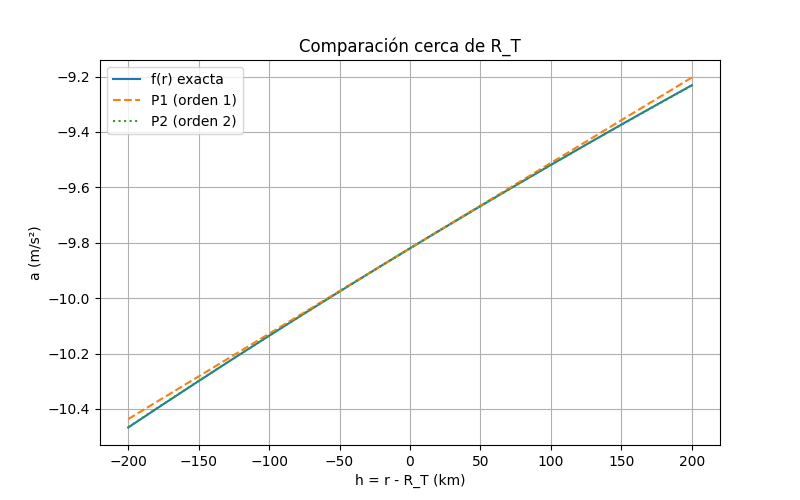
\includegraphics[width=1\textwidth]{assets/taylor_vs_gravedad.png}
    \caption{Gráfica de $r_0 = R_T$ y polinomio de Taylor de orden 2}
\end{figure}

\subsubsection{¿Cuánto debe alejarse un cuerpo para que g sea 1\% menor?}

Queremos encontrar la distancia $r$ tal que la aceleración gravitatoria disminuya un 1\% respecto a la que se experimenta en la superficie terrestre. Es decir:

\[
|f(R_T)| = \frac{GM}{R_T^2}, \quad \text{y queremos:} \quad \frac{GM}{r^2} = 0{,}99 \cdot \frac{GM}{R_T^2}
\]

Cancelando $GM$ en ambos lados de la ecuación:

\[
\frac{1}{r^2} = 0{,}99 \cdot \frac{1}{R_T^2} \quad \Rightarrow \quad r^2 = \frac{R_T^2}{0{,}99}
\]

\[
r = \frac{R_T}{\sqrt{0{,}99}} \approx 6\,403\,095\,\text{m}
\]

\[
h = r - R_T = 6\,403\,095 - 6\,371\,000 = 32\,096\,\text{m} \quad (\text{equivalente a } 32{,}1\,\text{km})
\]

\vspace{0.5em}

\textbf{Aproximación con el desarrollo de Taylor:}

Recordando que el cambio relativo en la aceleración se aproxima por:

\[
\Delta_{\text{rel}} \approx \frac{2h}{R_T} \quad \Rightarrow \quad h = \frac{\Delta_{\text{rel}} \cdot R_T}{2}
\]

Para $\Delta_{\text{rel}} = -0{,}01$:

\[
h \approx \frac{0{,}01 \cdot R_T}{2} = 0{,}005 \cdot R_T \approx 31\,855\,\text{m}
\]

\vspace{0.5em}

\textbf{Conclusión:} Se verifica que un cuerpo debe alejarse aproximadamente $32\,\text{km}$ de la superficie terrestre para que la aceleración gravitatoria sea un 1\% menor. Esta estimación es coherente tanto con el cálculo exacto como con la aproximación de Taylor.

\subsubsection{Radios 0,01 m y 0,02 m}

Analizamos la función de aceleración gravitatoria para radios extremadamente pequeños:

\[
f(r) = -\frac{GM}{r^2}
\]

Evaluando en $r = 0{,}01\,\text{m}$:

\[
f(0{,}01) = -\frac{GM}{(0{,}01)^2} = -\frac{GM}{1 \cdot 10^{-4}} = -GM \cdot 10^4
\]

Evaluando en $r = 0{,}02\,\text{m}$:

\[
f(0{,}02) = -\frac{GM}{(0{,}02)^2} = -\frac{GM}{4 \cdot 10^{-4}} = -\frac{GM \cdot 10^4}{4}
\]

\[
\Rightarrow \quad f(0{,}02) = \frac{1}{4} \cdot f(0{,}01)
\]

Se calcula la variación relativa de la aceleración gravitatoria al duplicar el radio desde $0{,}01\,\text{m}$ a $0{,}02\,\text{m}$:

\[
\Delta_{\text{rel}} = \frac{f(0{,}02) - f(0{,}01)}{f(0{,}01)} = \frac{\left(\frac{1}{4}f(0{,}01) - f(0{,}01)\right)}{f(0{,}01)} = -0{,}75
\]

\textbf{Interpretación:} La aceleración disminuye un $75\%$ al duplicar el radio.

\vspace{0.5cm}

\textbf{Desarrollo con polinomio de Taylor (orden 2) alrededor de $r_0 = 0{,}01\,\text{m}$}

\begin{align*}
f(r) &= -\frac{GM}{r^2} \\
f'(r) &= \frac{2GM}{r^3} \\
f''(r) &= -\frac{6GM}{r^4} \\
f^{(3)}(r) &= \frac{24GM}{r^5}
\end{align*}

Aplicando el polinomio de Taylor de segundo orden:

\[
P_2(r_0 + h) = f(r_0) + f'(r_0)h + \frac{f''(r_0)}{2}h^2
\]

Para $h = 0{,}01\,\text{m}$:

\[
P_2(2r_0) = -\frac{GM}{r_0^2} + \frac{2GM}{r_0^3} \cdot r_0 + \frac{-6GM}{2r_0^4} \cdot r_0^2
\]

\[
P_2(2r_0) = -\frac{GM}{r_0^2} + \frac{2GM}{r_0^2} - \frac{3GM}{r_0^2} = -\frac{2GM}{r_0^2}
\]

La aceleración predicha por Taylor de segundo orden a $r = 2r_0$ da una variación del $-0{,}25 \cdot f(r_0)$, es decir, una caída del $25\%$, lo cual difiere del valor real ($75\%$), evidenciando que el desarrollo de segundo orden no es suficiente para intervalos grandes.

Partimos del desarrollo de Taylor de orden 3 centrado en \( r_0 = 0{,}01\,\text{m} \):

\[
P_3(r_0 + h) = f(r_0) + f'(r_0) h + \frac{f''(r_0)}{2} h^2 + \frac{f^{(3)}(r_0)}{6} h^3
\]

Sabemos que:

\begin{align*}
f(r) &= -\frac{GM}{r^2} \\
f'(r) &= \frac{2GM}{r^3} \\
f''(r) &= -\frac{6GM}{r^4} \\
f^{(3)}(r) &= \frac{24GM}{r^5}
\end{align*}

Entonces, con \( h = r_0 \), se tiene:

\[
P_3(2r_0) = -\frac{GM}{r_0^2} + \frac{2GM}{r_0^2} - \frac{3GM}{r_0^2} + \frac{4GM}{r_0^2} = \frac{2GM}{r_0^2}
\]

\textbf{Interpretación:} El resultado obtenido al aplicar el polinomio de Taylor de orden 3 da un valor que cuadruplica el módulo del valor original de \( f(r_0) \), lo que indica que este desarrollo no es adecuado para estimar el valor de la función en un intervalo tan grande (de \( r_0 \) a \( 2r_0 \)). Este error significativo resalta que el desarrollo de Taylor tiene buena precisión únicamente en una cercanía al punto \( r_0 \).
También se observa que en el desarrollo de Taylor de orden 3, cambia de signo por lo cual se puede decir que en lugar de atraer, rechaza a los cuerpos, lo cual es físicamente incorrecto.

\subsubsection{Graficar r0 = 0.01 m para Polinomio de Taylor de orden 2 y 3}

\begin{figure}[H]
    \centering
    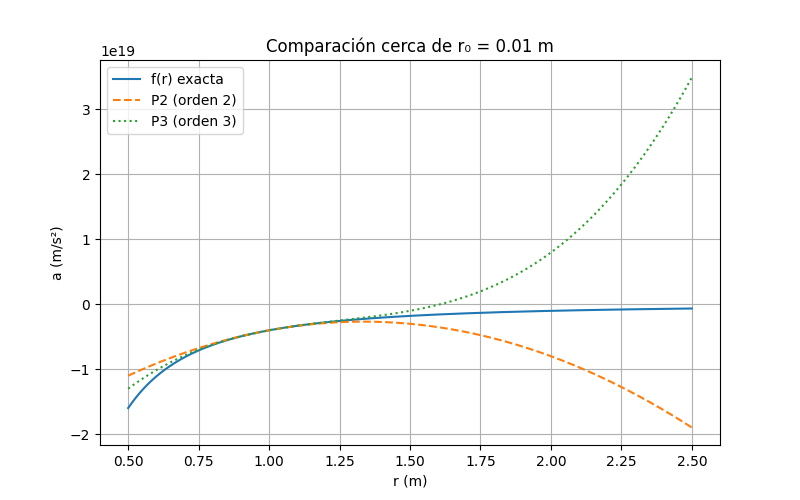
\includegraphics[width=1\textwidth]{assets/taylor_orden2y3.png}
    \caption{Gráfica de Taylor Orden 2 y 3 para $r_0 = 0.01$ m}
\end{figure}



\subsection*{Parte 2 – Caída con rozamiento}
\begin{enumerate}
\item Desarrollo de Taylor O(2) de $y(t)$; se discute la aceleración
inicial y el caso $\gamma\to0$.
\item Simulación numérica y superposición de curvas para los tres $\gamma$
(hormiga, persona, auto) y las seis combinaciones .
\item Obtención analítica de la velocidad terminal
$v_T=-\dfrac{g}{\gamma}$ y verificación en las simulaciones.
\item Criterio basado en $\gamma t\ll1$ para descartar la resistencia.
\end{enumerate}
Los resultados se comentan sobre cada gráfico generado por
\codeword{caida_con_rozamiento.py}.

% --------------------------------------------------------------------
\section{Conclusiones}\label{sec:conclusiones}
\begin{itemize}
\item Los polinomios de Taylor orden 1 y 2 son suficientes para aproximar
la ley $,-GM/r^2$ a menos de 0.3 % en la baja atmósfera.
\item En el modelo con rozamiento lineal, el término adicional
$\tfrac12\gamma v_0 t^2$ delimita la validez de la aproximación.La condición $\gamma t<0.3$ (<10 % de corrección) resultó un umbral
práctico en todas las simulaciones.
\item El uso del Taylor permitió justificar algebraicamente cuándo las
curvas con y sin aire se separan, antes de siquiera integrar
numéricamente el sistema.
\end{itemize}

% --------------------------------------------------------------------
\section{Referencias}
\begin{enumerate}
\item Suárez, J. E., \& González, M. A. (2018). Polinomios de Taylor: teoría y aplicaciones. \textit{Revista Iberoamericana de Matemática, 35}(2), 123–145.
\item Serway, R.
\emph{Física para ciencias e ingeniería}. Cengage Learning.
\item Notas de curso de Cálculo Aplicado – UCU (2024).
\end{enumerate}
\section{Referencias}
Suárez, J. E., \& González, M. A. (2018). Polinomios de Taylor: teoría y aplicaciones. \textit{Revista Iberoamericana de Matemática, 35}(2), 123–145.

Stewart, J. (2015). \textit{Cálculo de una variable} (7ª ed.). Cengage Learning.

\end{document}